\documentclass[a4paper,12pt]{article}
\usepackage{../packages/coursCollege}
\newcommand{\Chapitre}{Ch. 3: Fonctions}
\renewcommand{\path}{../}
\usepgfplotslibrary{fillbetween}

\usepackage[    %backend=biber,
    natbib=true,
    style=numeric,
    sorting=none]{biblatex}  % Load biblatex for bibliography handling
\addbibresource{biblio-der.bib}
\renewcommand\refname{Sources}
\renewcommand{\cours}{1MA~--~EG~--~ns~--~2025-2026}
% Define the style within pgfplotsset to avoid namespace errors
\pgfplotsset{
    artistic_axis/.style={
        axis lines=middle,
        grid=both,
        grid style={line width=.1pt, draw=gray!15},
        major grid style={line width=.2pt, draw=gray!30},
        ticks=none,
        xlabel style={at={(ticklabel* cs:1)}, anchor=north west},
        ylabel style={at={(ticklabel* cs:1)}, anchor=south west},
        font=\small
    }
  }

  \begin{document}
\tocloftpagestyle{fancy}
% Reduce space between section entries
\setlength{\cftbeforesecskip}{2pt}

% Reduce indentation for section entries
\setlength{\cftsecindent}{1em}

\begin{center}
	{\bfseries \Huge Chapitre 3 : Fonctions}

% Side-by-side individual plots using the tasks package
\begin{tasks}(4)
    \task[]
    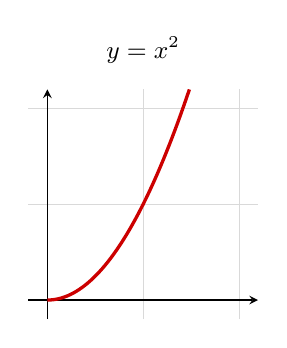
\begin{tikzpicture}
        \begin{axis}[artistic_axis, width=4.5cm, height=4.5cm, xmin=-0.2, xmax=2.2, ymin=-0.2, ymax=2.2, title={$y=x^2$}]
            \addplot[very thick, red!80!black, domain=0:sqrt(2.2), samples=50] {x^2};
        \end{axis}
    \end{tikzpicture}

    \task[]
    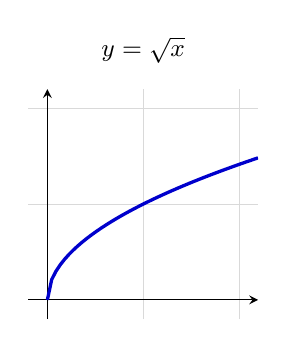
\begin{tikzpicture}
        \begin{axis}[artistic_axis, width=4.5cm, height=4.5cm, xmin=-0.2, xmax=2.2, ymin=-0.2, ymax=2.2, title={$y=\sqrt{x}$}]
            \addplot[very thick, blue!80!black, domain=0:2.2, samples=50] {sqrt(x)};
        \end{axis}
    \end{tikzpicture}

    \task[]
    \begin{tikzpicture}
        \begin{axis}[artistic_axis, width=4.5cm, height=4.5cm, xmin=-0.2, xmax=2.2, ymin=-0.2, ymax=2.2, title={$y=\dfrac{1}{x}$}]
            \addplot[very thick, orange!80!black, domain=0.45:2.2, samples=50] {1/x};
        \end{axis}
    \end{tikzpicture}

    \task[]
    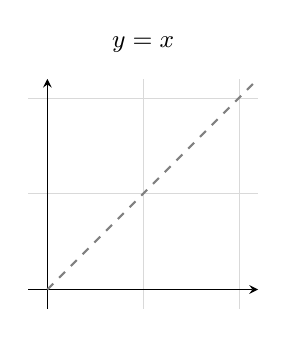
\begin{tikzpicture}
        \begin{axis}[artistic_axis, width=4.5cm, height=4.5cm, xmin=-0.2, xmax=2.2, ymin=-0.2, ymax=2.2, title={$y=x$}]
            \addplot[thick, gray, dashed, domain=0:2.2] {x};
        \end{axis}
    \end{tikzpicture}
\end{tasks}


\pgfplotsset{
    transformation_plot/.style={
        axis lines=middle,
        xmin=-4, xmax=4,
        ymin=-2, ymax=6,
     xtick={-4,-3,...,4},
    ytick={-2,-1,...,6},
        grid=both,
        grid style={line width=.1pt, draw=gray!15},
        major grid style={line width=.2pt, draw=gray!30},
        ticks=none,
        width=4.5cm, height=4.5cm,
        font=\small,
        every axis plot/.append style={very thick, cyan!70!black}
    }
}

\begin{tasks}(4)
    % 1. Parent Function
    \task[]
    \begin{tikzpicture}
        \begin{axis}[transformation_plot, title={$y=x^2$}]
            \addplot[domain=-2.4:2.4, samples=50] {x^2};
        \end{axis}
    \end{tikzpicture}

    % 2. Vertical Shift
    \task[]
    \begin{tikzpicture}
        \begin{axis}[transformation_plot, title={$y=x^2+2$}]
            \addplot[domain=-2:2, samples=50] {x^2+2};
        \end{axis}
    \end{tikzpicture}

    % 3. Vertical Compression
    \task[]
    \begin{tikzpicture}
        \begin{axis}[transformation_plot, title={$y=\dfrac{1}{2}x^2$}]
            \addplot[domain=-3.4:3.4, samples=50] {0.5*x^2};
        \end{axis}
    \end{tikzpicture}

    % 4. Horizontal Shift
    \task[]
    \begin{tikzpicture}
        \begin{axis}[transformation_plot, title={$y=(x-2)^2$}]
            \addplot[domain=-0.4:4, samples=50] {(x-2)^2};
        \end{axis}
    \end{tikzpicture}

    % 5. Combined Transformation
    \task[]
    \begin{tikzpicture}
        \begin{axis}[transformation_plot, title={$y=\dfrac{1}{2}(x-2)^2+1$}]
            \addplot[domain=-1:4, samples=50] {0.5*(x-2)^2+1};
        \end{axis}
    \end{tikzpicture}

    % 6. Reflection
    \task[]
    \begin{tikzpicture}
        \begin{axis}[transformation_plot, title={$y=-x^2$}]
            \addplot[domain=-2.4:2.4, samples=50] {-x^2};
        \end{axis}
    \end{tikzpicture}

    % 7. Vertical Stretch
    \task[]
    \begin{tikzpicture}
        \begin{axis}[transformation_plot, title={$y=2x^2$}]
            \addplot[domain=-1.7:1.7, samples=50] {2*x^2};
        \end{axis}
    \end{tikzpicture}

    % 8. Multiple Shifts and Reflection
    \task[]
    \begin{tikzpicture}
        \begin{axis}[transformation_plot, title={$y=-(x+1)^2+3$}]
            \addplot[domain=-3.5:1.5, samples=50] {-(x+1)^2+3};
        \end{axis}
    \end{tikzpicture}
\end{tasks}
\end{center}

\vspace{-1cm}

\tableofcontents

\newpage
\section{Généralités sur les fonctions}
\subsection{Découverte de quelques fonctions et vocabulaire}
\insertexo{n6f5f}{false}{exo}
\insertexo{qcb47}{false}{exo}
\insertexo{xd937}{false}{exo}
\insertexo{m6328}{false}{exo}


\insertexo{b6cb8}{false}{exo}
\insertexo{b2603}{false}{exo}
\insertexo{lfcbb}{false}{exo}
\insertexo{z0962}{false}{exo}
\insertexo{v54f9}{false}{exo}
\insertexo{cb3da}{false}{exo}
\insertexo{c1e38}{false}{exo}
\insertexo{f8be0}{false}{exo}
\insertexo{u3450}{false}{exo}
\insertexo{i705d}{false}{exo}
\subsection{Domaine de définition}
\insertexo{cd938}{false}{exo}
\insertexo{m167b}{false}{exo}
\insertexo{q7bcb}{false}{exo}
\insertexo{v3d78}{false}{exo}
\insertexo{k0236}{false}{exo}
\insertexo{h4652}{false}{exo}
\insertexo{u1722}{false}{exo}
\subsection{Opérations sur les fonctions}
\insertexo{d7ab2}{false}{exo}
\insertexo{tcbf7}{false}{exo}
\insertexo{adb2d}{false}{exo}
\subsection{Composition de fonctions}
\insertexo{f6d6b}{false}{exo}
\insertexo{s13bb}{false}{exo}
\insertexo{k33be}{false}{exo}
\insertexo{je439}{false}{exo}
\insertexo{jd7da}{false}{exo}
\insertexo{c688a}{false}{exo}
\insertexo{k3146}{false}{exo}
\insertexo{f02af}{false}{exo}
\insertexo{l5835}{false}{exo}
\insertexo{v91bb}{false}{exo}
\insertexo{pbb73}{false}{exo}
\insertexo{wb9ff}{false}{exo}
\section{La droite}
\subsection{Représentation}
\insertexo{b8eb6}{false}{exo}
\insertexo{a5561}{false}{exo}
\insertexo{ua665}{false}{exo}
\insertexo{u082f}{false}{exo}
\insertexo{o3a87}{false}{exo}
\insertexo{d775a}{false}{exo}
\insertexo{pa02f}{false}{exo}
\insertexo{fa8ff}{false}{exo}
\insertexo{b2e74}{false}{exo}
\insertexo{acc7c}{false}{exo}
\insertexo{y3eae}{false}{exo}
\insertexo{h8fbd}{false}{exo}
\insertexo{l368d}{false}{exo}
\insertexo{t3d16}{false}{exo}
\insertexo{x1fab}{false}{exo}
\insertexo{u416d}{false}{exo}
\insertexo{u5d18}{false}{exo}
\subsection{Droites parallèles et perpendiculaires}
\insertexo{of723}{false}{exo}
\insertexo{b2bfd}{false}{exo}
\insertexo{fcacb}{false}{exo}
\insertexo{lc23a}{false}{exo}
\insertexo{jf835}{false}{exo}
\insertexo{t4cab}{false}{exo}
\insertexo{u06a8}{false}{exo}
\insertexo{x844f}{false}{exo}
\section{La parabole}
\subsection{Définitions et différentes formes}
\insertexo{jb01e}{false}{Exo}
\insertexo{a2371}{false}{exo}
\insertexo{sc0ae}{false}{exo}
\insertexo{x1384}{false}{exo}
\insertexo{n3d9e}{false}{exo}
\insertexo{af4d2}{false}{exo}

\subsection{Extremum}
\insertexo{i34c4}{false}{exo}
\insertexo{f5f9a}{false}{exo}
\insertexo{z8537}{false}{exo}
\insertexo{cc016}{false}{exo}
\insertexo{h2451}{false}{exo}
\insertexo{h5627}{false}{exo}

\subsection{Intersections}
\insertexo{h3c4c}{false}{exo}
\insertexo{lf2a1}{false}{exo}
\insertexo{pc233}{false}{exo}
\insertexo{p5deb}{false}{exo}
\subsection{Optimisation}
\insertexo{efc34}{false}{exo}
\insertexo{x07dc}{false}{exo}
\insertexo{x8166}{false}{exo}
\insertexo{u4adb}{false}{exo}
\insertexo{ne2ae}{false}{exo}
\insertexo{bf450}{false}{exo}
\end{document}
